\documentclass[12pt,letterpaper,noanswers]{exam}
\usepackage[usenames,dvipsnames,svgnames,table]{xcolor}
\usepackage[margin=0.9in]{geometry}
\renewcommand{\familydefault}{\sfdefault}
\usepackage{multicol}
\pagestyle{head}
\definecolor{c03}{HTML}{FFDDDD}
\header{AM 108 Class 14}{}{limit cycle}
\runningheadrule
\headrule
\usepackage{graphicx} % more modern
\usepackage{amsmath} 
\usepackage{amssymb} 
\usepackage{hyperref}
\usepackage{tcolorbox}

\begin{document}
 \pdfpageheight 11in 
  \pdfpagewidth 8.5in

\noindent 




\begin{itemize}
    \item There is a problem set due Friday October 9th.
    \item By default, the quiz follow up is due on Monday (note that there is not class on Monday).  However, it can be due a different day - contact me via private message on Piazza.
    \item There is a skill check in class on Friday.  The problem info is below.
\end{itemize}

\hrule
\vspace{0.2cm}





\noindent\textbf{Teams}

\begin{multicols}{2}
1. 
\end{multicols}

\noindent \textbf{Teams 5 and 6}: Post screenshots of your work to the course Google Drive today.  Include words, labels, and other short notes that might make those solutions useful to you or your classmates.  Find the link in Canvas (or here: \url{https://drive.google.com/drive/u/0/folders/1GcpwvKHD4tMecpFQ4lNxN_r5Ylj7YHbd})

\vspace{0.2cm}

\hrule
\vspace{0.2cm}

\noindent\textbf{Big picture}

We have been learning methods for constructing a phase portrait for a 2d system.  Today we are using the Poincar\'e-Bendixson theorem to rule in closed trajectories as part of a phase portrait.


\noindent \textbf{Extra vocabulary / extra facts:}
\begin{tcolorbox}
A \textbf{closed} set is a set that contains its own boundary.  The trapping region we construct in the Poincar\'e-Bendixson theorem is a closed and bounded subset of the plane.

\textbf{}
\end{tcolorbox}

\begin{center}
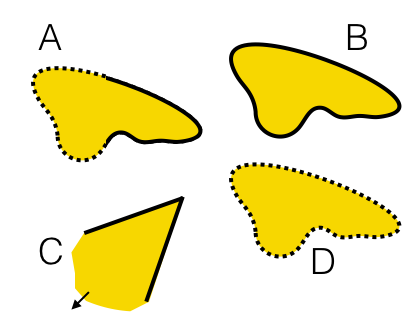
\includegraphics[width=3in]{img/C15p2.png}
\end{center}

% \vspace{0.2cm}

% \hrule
% \vspace{0.2cm}

$B$ is a closed and bounded set.  $D$ is an open and bounded set.  $C$ is closed but unbounded.  $A$ is neither open nor closed and is bounded.

\vspace{0.2cm}

\hrule
\vspace{0.2cm}

\noindent\textbf{Your questions}
\begin{enumerate}
    \item Why can't linear systems have limit cycles?  What is the difference between a limit cycle and a closed trajectory or between a limit cycle and a periodic solution?
    \item How would we use the Poincar\'e-Bendixson theorem when there are multiple fixed points?
    \item To show that all vectors on the boundaries of a region point inward would it be possible to use a line integral or a flux integral?
    \item In the Poincar\'e-Bendixson theorem, we need to show that there is a trapped trajectory in $R$ for all $t\geq t_0$.  Can trajectories originating from an unstable fixed point be within $R$ for all $t\geq t_0$, including $t = t_0$?
    \item To find a bounding region, Steve used an approximation to the vector field when $x,y\gg 1$.  How do people choose these kinds of cases for approximation?  Will it be specific to the system?
\end{enumerate}

\vspace{0.2cm}
\hrule
\vspace{0.2cm}


\noindent\textbf{Skill Check C15 practice}
\begin{questions}
\item Retake of skill check C12 on finding $\frac{dE}{dt}$ along trajectories for a given $E(x,y)$ and given dynamical system.

\item Consider a dynamical system specified by $\dot r = r(2-\sin\theta/2 -r)$, $\dot\theta = 1$, with the phase portrait below.  Use $\dot r$ to identify inequalities that define a trapping region that satisfies the conditions of the Poincar\'e-Bendixson theorem.


\emph{The gridlines are drawn with an interval of $1$ units.}


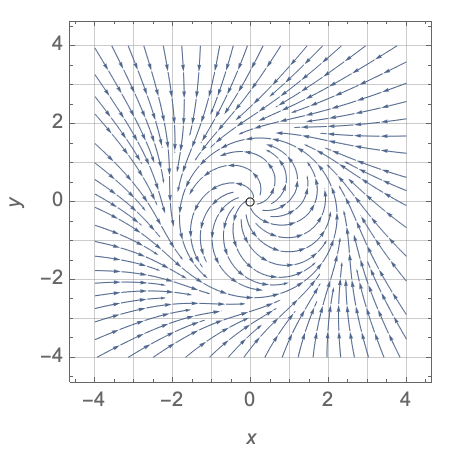
\includegraphics[]{img/C14-C15trapping.png}

\vspace{0.2cm}

\hrule
\vspace{0.2cm}
\end{questions}



\noindent\textbf{Skill check C15 practice solution}

We're using polar coordinates for this. $\dot\theta >0$, so there will be no fixed points away from the origin.  I have $\dot r = r(2-\sin\theta/2-r)$.  For $r$ large, $2-\sin\theta/2 -r < 0$.  Specifically, $2-\sin\theta/2$ has a max of $2.5$ so for $r = 3$ we have $\dot r < 0$.  In addition, $2-\sin\theta/2\geq 1.5$ so for $r = 1$ we have $\dot r > 0$

I choose $1 \leq r \leq 3$.  This is a closed region (the $=$ in the $\leq$ means it includes its boundary), excludes the fixed point at the origin, and (based on my observations about the sign of $\dot r$ above), has all vectors pointing into the region along the boundaries.


\vspace{0.2cm}
\hrule
\vspace{0.2cm}





\eject



\vspace{0.2cm}

\hrule
\vspace{0.2cm}

\begin{questions}
  
% \question
% \begin{parts}
% \item Like last time, sketch a phase portrait for a system with a saddle point at the origin.
% \item Now add a stable spiral at $(1,0)$.  Connect the two local pictures up by having an (appropriate) unstable manifold of your saddle point spiral into the stable spiral.
% \item Could a closed trajectory exist in this system?  If so, where? 
% \end{parts}



\question (Constructing a trapping region). Use the nullclines and the vector field to help you to construct a trapping region that satisfies the conditions of the Poincar\'e-Bendixson theorem.  (Assume this system has an unstable fixed point.)

\emph{This is not easy to do but should be possible}

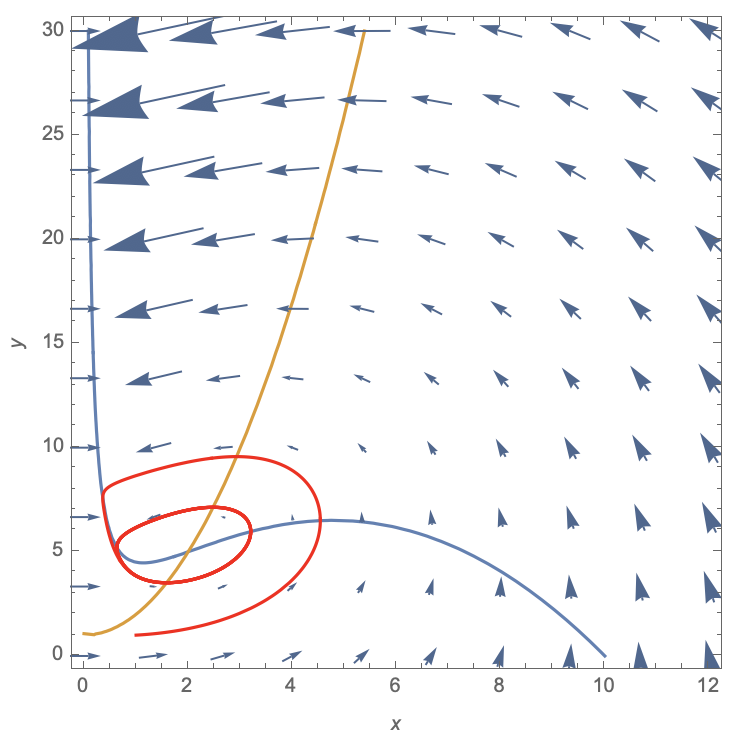
\includegraphics{img/C14trappingp1.png}




\question (Working in polar) Using polar coordinates can be a straightforward way to make a system that is constructed to have closed orbits.

Consider the system
\begin{align*}
\dot{r} = &\  r(1-r)(2-r) \\
\dot{\theta} = &\ 1.
\end{align*}

\begin{parts}
\item We'll think about this system in the $xy$-plane.  Note that $\dot{\theta} = 1$ so $\theta(t) = (t+\theta_0)$, and we think of it mod $2\pi$.  The angle is continuously increasing in the counterclockwise direction.  This continuous motion in the angle means that, away from the origin, there can't be a fixed point.  
\begin{itemize}
\item What kind of trajectory will you have for this system when $\dot{r} = 0$?
\item What about if $\dot{r}= 0$ and $r = 0$?
\end{itemize}
\item To analyze the system, first consider the 1d system
\[\frac{dx}{dt} = x(1-x)(2-x).\] 
What are the fixed points?  Sketch what is happening on the $x$-axis.  Restrict yourself to $x\geq 0$.
\item Now think about the system 
\begin{align*}
\dot{r} = &\  r(1-r)(2-r) \\
\dot{\theta} = &\ 1.
\end{align*}
Sketch in the $\dot{r} = 0$ trajectories.  Try to sketch a phase portrait.
\end{parts}


\question (Constructing a trapping region) 

Consider the system 
\begin{align*}
\dot{r} = &\  r(2-\sin\theta -r) \\
\dot{\theta} = &\ 1.
\end{align*}

\begin{parts}
\item Argue that the curve $r = 2-\sin\theta$ does not exactly correspond to a trajectory of the system.
\item For $r = 4$, identify the minimum and maximum possible values of $\dot r$ that could occur.
\item Construct a trapping region that satisfies the conditions of the Poincar\'e-Bendixson theorem.
\end{parts}


\end{questions}

\eject
\textbf{Answers}:

% 1a: sketch of a saddle: two unstable directions, two stable ones, and those curvy trajectories.

% 1b: \includegraphics[width=4in]{img/S19C13p1.png}  Other configurations of the saddle point are possible, as is another orientation to the spin of the spiral.

% 1c: saddle point: index $-1$.  spiral: index $+1$.  both: index $0$.  So a closed trajectory would have to enclose just the spiral for the index to work out.  That isn't possible, because it would have to cross the unstable manifold of the saddle to do that.  No closed trajectories in this system!

1: %I believe my line segments are oriented so that all of the vectors go inward.  I haven't found the vector field on each line to compare the slopes, though, so I'm not positive...

%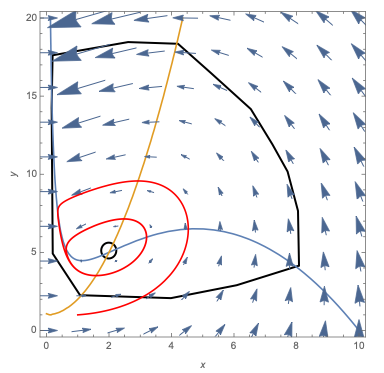
\includegraphics{img/C15_2019_10_07_p4.png}

2a: $\dot{r} = 0$ and $\dot{r} = 0$ is a fixed point; just $\dot{r} = 0$ is a closed orbit.

2b: fixed points at $0, 1, 2$.  At $x=3$, $\frac{dx}{dt} = 3(-2)(-1) > 0$ so $2$ is unstable, $1$ is stable, $0$ is unstable.  

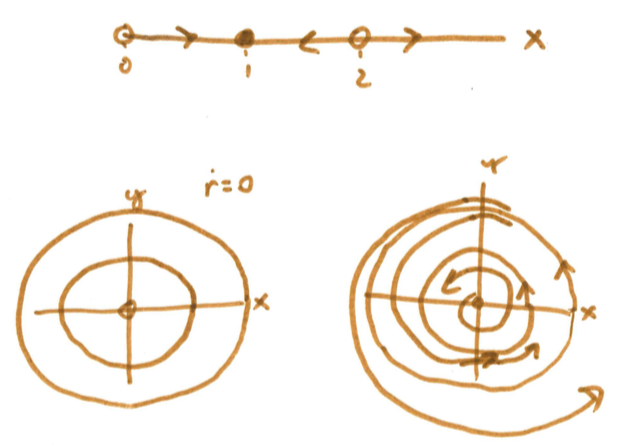
\includegraphics[width=4in]{img/S19C13p2.png}

2c: 

3a: The curve $r = 2-\sin\theta$ is wiggly: it doesn't have a constant radius.  So I'll move off of it because of the $\dot\theta = 1$ contribution.

3b: $\dot r$ ranges from $4(2-1-4)=4(-3)=-12$ to $4(2+1-4)=4(-1)=-4$.  It is always negative.

3c: $\dot r>0$ for all $\theta$ when $r = 0.5$ so $0.5\leq r\leq 4$ is a trapping region.  There are no fixed points away from $r=0$ so there are no fixed points within the region.

\end{document}